\section{Systementwurf}

\subsection{Modellierung der Datenbank}

Um die Daten zu modellieren ist es sinnvoll, sich diese im Kontext der Erhebung zu betrachten. In (\ref{eq:datenstruktur}) ist dieser Prozess vereinfacht dargestellt.

\begin{equation}
    \mbox{Boje} \to (\mbox{misst}_{\mbox{an Ort}}) \to \mbox{Messprofile}\label{eq:datenstruktur}
\end{equation}

Dabei ist erkennbar, dass dieses Modell eine Verkettung von Entitäten und Ereignissen darstellt. Eine Boje misst über ihre Lebensdauer eine Anzahl von Messzyklen. Jeder dieser Messzyklen besteht aus einer gewissen Anzahl von Messwerten.

Um das Modell weiter fortzuführen, wurde diese Ereigniskette in ein Entitätsschema überführt. In Abbildung \ref{fig:ERM} ist die hier verwendete Modellierung des Prozesses zu sehen.

\begin{figure}[h!]
    \centering
    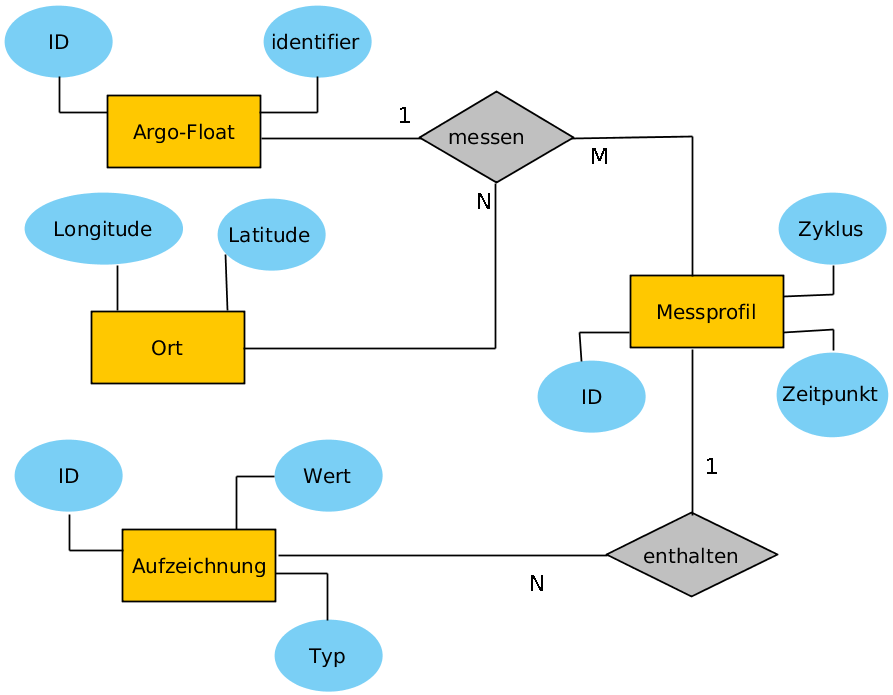
\includegraphics[width=0.6\textwidth,clip=true,trim=0pt 0pt 0pt 0pt]{pix/erm.png}
    \caption{Beschreibung der Entitäten der Datenaggregation}
    \label{fig:ERM}
\end{figure}


\subsection{Architektur}


Wie in Abbildung \ref{fig:grobetwurf_architektur_datenaggregation} zu sehen ist, besteht die Applikation aus zwei Grundkomponenten. Der erste Teilbereich ist für die Beschaffung und Aufbereitung der Daten zuständig, während der zweite Teilbereich für die Darstellung der Daten zuständig ist.

% BEGIN OOP ARCHITEKTUR   AGGREGATION
\subsubsection{Entwurf der Datenaggregation}\label{sec:entwurfAggregation}
\begin{figure}[h!]
\centering
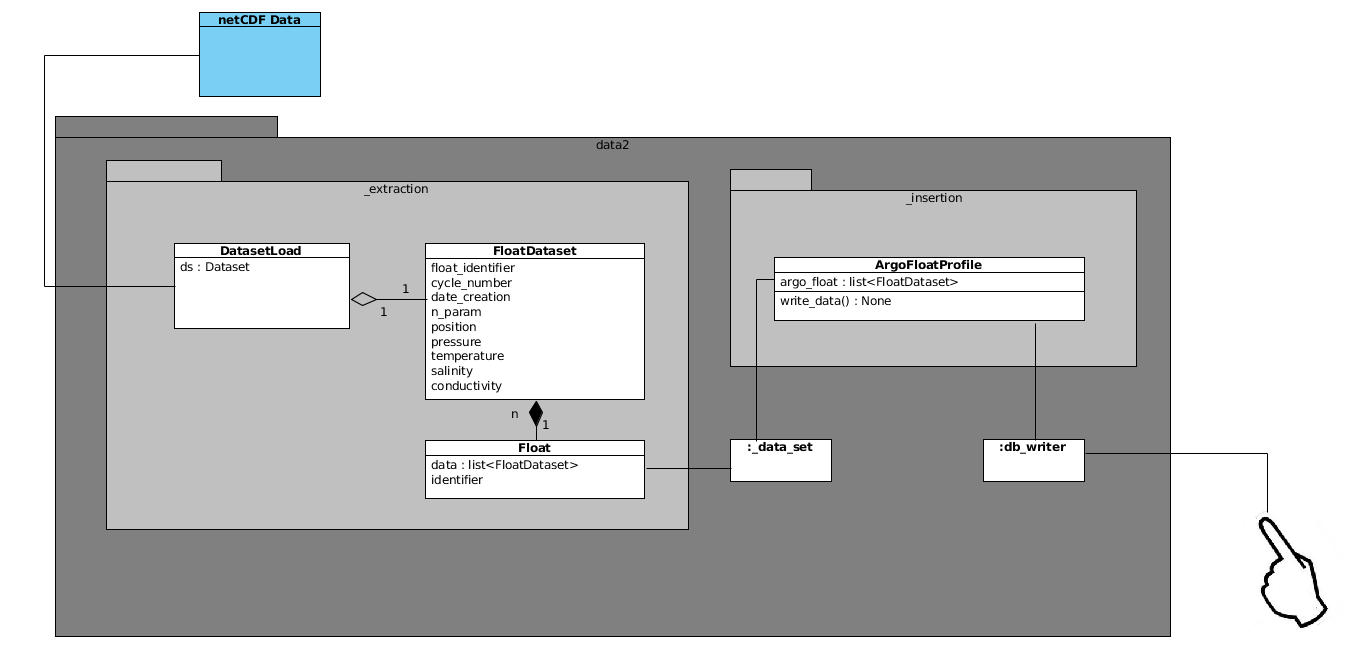
\includegraphics[width=\textwidth]{pix/grobentwurf_dataaggregation.png}
% grobentwurf_dataaggregation.png: 1436x727 px, 96dpi, 37.99x19.23 cm, bb=
\caption{Entwurf der Architektur der Aggregation der Daten}
\label{fig:grobetwurf_architektur_datenaggregation}
\end{figure}

Die Datenaggregation erfüllt zwei Funktionen. Zum einen muss sichergestellt sein, dass die Daten aus den vom Argo-Programm bereitgestellten Strukturen gelesen und in ein logisches Format überführt werden. Des Weiteren müssen diese Daten in die Datenbank der Applikation überführt werden.

Auch in diesem Modell ist die Ereigniskette aus (\ref{eq:datenstruktur}) abzubilden. Jede Messstation wird über ein Objekt abgebildet. Die hier gespeicherten Daten sind für eine Messstation eindeutig. Jeder Messzyklus der Boje wird über ein weiteres, zur Messstation gehöriges Objekt abgebildet. Dieses ist innerhalb des Kontextes eindeutig und trägt die Informationen zur jeweiligen Messung.

Für die Persistierung  werden objektorientierte Strukturen für den ORM verwendet. Diese Strukturen teilt sich das Modul mit der Webapplikation. Die Behandlung der Daten sowie eine Steuerung des Prozesses sind als weitere Schnittstellen zu definieren.

Die Aggregation der Daten wird über zwei Teilbereiche abgebildet. Zum einen müssen die benötigten Parameter aus den Dateien ausgelesen und modelliert werden.
Als zweite Ebene der Aggregation ist der Prozess des Schreibens in eine Datenbank zu sehen. Diese verwendet die zuvor ermittelten modellierten Messprofile und schreibt sie Anhand der dort enthaltenen Daten in eine Datenbank.


Es ist an dieser Stelle zu erkennen, dass zwei Stellen existieren, die die intrinsischen Eigenschaften des Modules an dieser Stelle beeinflussen. Im folgenden werden die Schnittstellen aufgelistet, die eine richtige Handhabung festsetzen:

\paragraph{Schnittstellen}

\begin{enumerate}

\item \textbf{Daten}
    \begin{enumerate}
        \item Die Datenstruktur ist normiert. Es ist sicherzustellen, dass die bekannte Daten- bzw. Ordnerstruktur abgearbeitet wird. Mit Änderungen in dieser Struktur muss nicht gerechnet werden.
        \item Es muss sicher gestellt werden, dass geöffnete Dateien wieder geschlossen werden.
    \end{enumerate}

\item \textbf{Steuerung}
    \begin{enumerate}
        \item Daten separiert in die Datenbank zu schreiben, könnte zu Inkonsistenzen führen und soll vermieden werden.
        \item Der Prozess sollte als Sequenz modelliert werden.
        \item Es muss sicher gestellt werden, dass die Daten schrittweise in die Datenbank überführt werden. Würden zu Beginn alle Dateien geöffnet und gemeinsam im flüchtigen Speicher vorgehalten, könnte es zu Problemen führen.
    \end{enumerate}

\end{enumerate}

% END

% BEGIN OOP ARCHITEKTUR   WEBAPPLIKATION

\subsubsection{Entwurf der Webapplikation}

Die Webapplikation besteht aus zwei Teilkomponenten. Die erste Komponente ist für die Darstellung der Webseite zuständig (app). Durch diese werden Elemente in  HTML, Javascript und als Bilder ausgeliefert, welche im Webbrowser den Benutzenden angezeigt werden können. Die Darstellung erfolgt dabei dem Singlepage-Prinzip.

Die zweite Teilkomponente ist dafür zuständig, benötigten Daten bereitzustellen (api). Alle Daten aus der Datenhaltung werden über diese Schnittstelle angefordert. Die Daten werden über JSON codiert.


\subsubsection{Ausarbeitung der Webrouten} \label{sec:entwurfRoutes}


Die \textbf{api} ist dafür zuständig, die benötigten Daten der Applikation bereitzustellen. Über definierte Webrouten wird über einen GET-Request ein JSON angefordert. Die  hierfür ausgearbeitete Struktur ist in Listing \ref{lst:routesAPI} zu sehen und ist im Folgenden beschrieben:

\begin{python}[label={lst:routesAPI}, caption={Webrouten der Datenrepresentation}]
(1.1) GET     /last_seen
(1.2) GET     /last_seen/[force_reload]
(1.3) GET     /argo_float/[identifier]
(1.4) GET     /positions/[identifier]
\end{python}

\begin{description}
 \item [(1.1) / (1.2)]
    Über diese Route  werden die Daten für die letzte Position der Messstationen aufgerufen. Dieser Datensatz trägt die Daten, die zur Anzeige der Positionen der Messstationen auf der Weltkarte benötigt werden und die Zusatzinformationen zur Darstellung eines Tooltips der einzelnen Argo-Floats. Die Daten werden bei jedem Besuch der Webseite ausgeliefert. Da sich diese erst verändern, wenn neue Daten vorliegen, werden diese über einen Caching-Mechanismus vorgehalten. Der optionale Übergabeparameter \texttt{force\_reload} ermöglicht das Neuanlegen des Caches. Um Vandalismus vorzubeugen, sollte es sich dabei um einen nicht zu  erratenden Token handeln.

 \item [(1.3)]
    Über diese Route werden die Mess-, wie auch Metadaten einer Messstation angefordert. Die Auswahl der Boje erfolgt über den Übergabeparameter \texttt{identifier}. Hier wird die eindeutige Identifikationsnummer  (siehe PLATTFORM\_NUMBER in Tabelle \ref{table:Datenauswahl}) der Messstation verwendet.

 \item [(1.4)]
    Um den Positionsverlauf einer Boje anzufordern, dient diese Route. Auch hier wird zur Identifikation der Messstation deren Identifikationsnummer als Parameter übergeben.
\end{description}



Die \textbf{app} liefert die Teile aus, die vom Benutzer gesehen werden. Es handelt sich dabei um HTML/Javascript und Bilddaten. Die hierfür ausgearbeitete Struktur ist in Listing \ref{lst:routesAPP} zu sehen und im Folgenden beschrieben:

\begin{python}[label={lst:routesAPP}, caption={Webrouten der Darstellung}]
(2.1) GET     /
(2.2) GET     /chart/[identifier]
(2.3) GET     /info/[identifier]
\end{python}

\begin{description}
 \item [(2.1)]
 Über diese Seite ist die eigentliche Applikation zu sehen. Dies umfasst die Karte sowie die angezeigten Messwerte.

 \item [(2.2)]
 Diese Route stellt den Plot der darzustellenden Messwerte als Bild zur Verfügung.

 \item [(2.3)]
 Über diese Route wird ein HTML für die Infoanzeige einer Messstation bereitgestellt.

\end{description}


% END

% BEGIN DESIGN DARSTELLUNG
\subsubsection{Aussehen der Webapplikation}
%
%
% - Darstellung der Daten -- ...

\begin{figure}[h!]
    \centering
    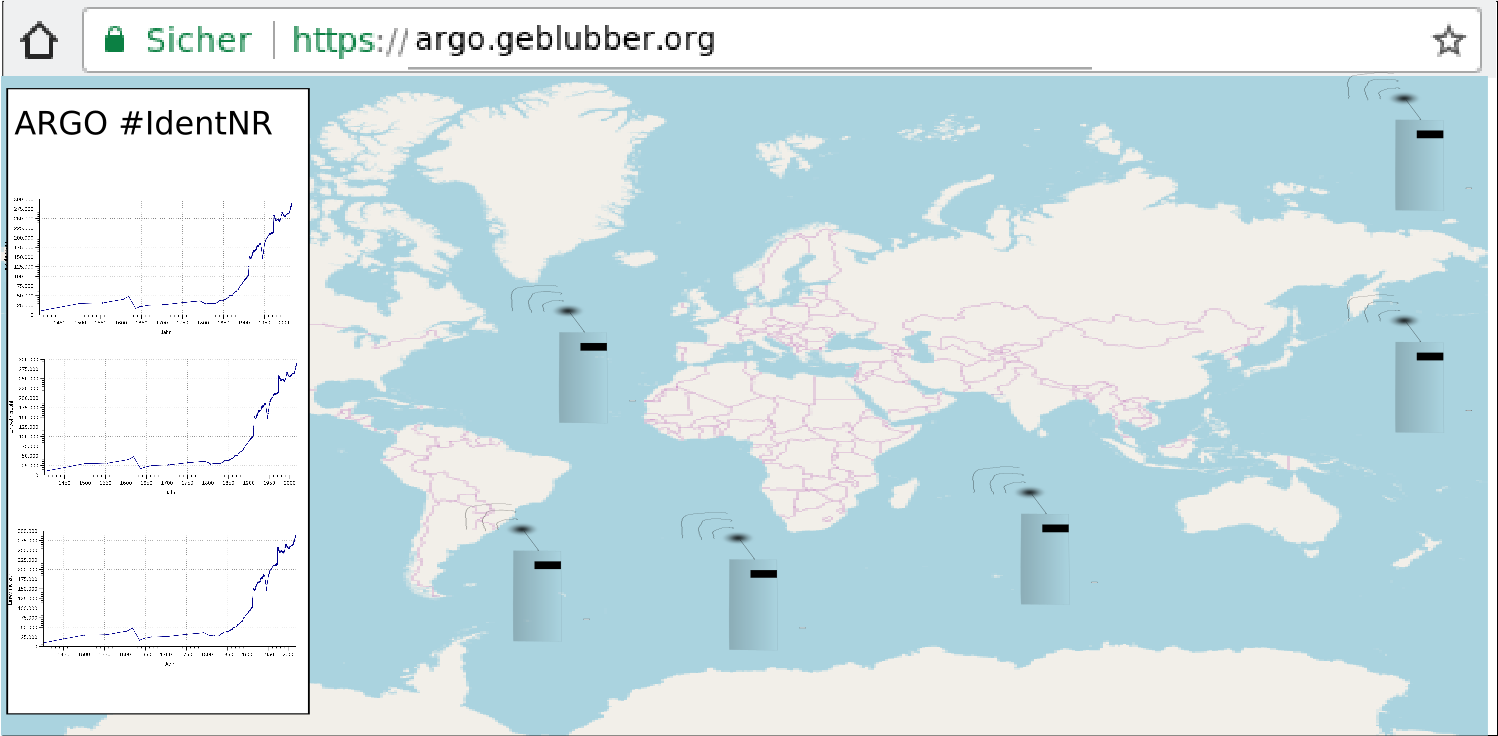
\includegraphics[width=\textwidth]{pix/EntwurfWebseite.png}
    % Entwurf_Webseite.svg.png: 1498x736 px, 96dpi, 39.63x19.47 cm, bb=0 0 1123 552
    \caption{Grafischer Grobentwurf der Webapplikation}
    \label{fig:entwurf_webseite}
\end{figure}

Das Aussehen der Applikation soll dem Muster von gängigen Webapplikationen entsprechen. In Abbildung \ref{fig:entwurf_webseite} ist ein erster Grobentwurf der Applikation zu sehen.
Zentrales Element der Applikation ist die Darstellung einer Karte. Über diese sollen die letzten Positionen der Karte ersichtlich sein.
Klickt man eine Messstation an, so wird auf der linken Seite ein weiteres Element in die Seite eingefügt. Dieses dient zur Darstellung der Messwerte des jeweiligen Argo-Floats.





% END
